\documentclass[conference]{IEEEtran}
\IEEEoverridecommandlockouts
\usepackage{cite}
\usepackage{amsmath,amssymb,amsfonts}
\usepackage{algorithmic}
\usepackage{graphicx}
\usepackage{textcomp}
\usepackage{xcolor}
\usepackage{float}
\def\BibTeX{{\rm B\kern-.05em{\sc i\kern-.025em b}\kern-.08em
    T\kern-.1667em\lower.7ex\hbox{E}\kern-.125emX}}
\begin{document}

\title{Time Series Analysis of Monkeypox Virus Cases and Prediction in Mexico\\
}

\author{\IEEEauthorblockN{José Eduardo Zarate Aranda}
\IEEEauthorblockA{\textit{School of Engineering and Science} \\
\textit{Tecnologico de Monterrey}\\
Guadalajara, Mexico \\
A01630299@tec.mx}
\and
\IEEEauthorblockN{Farid Jacome Velasco}
\IEEEauthorblockA{\textit{School of Engineering and Science} \\
\textit{Tecncologico de Monterrey}\\
Ciudad de México, México \\
A01654534@tec.mx}
}

\maketitle

\begin{abstract}
The monkeypox virus causes a zoonotic disease that infects animals and humans; the outbreak was confirmed in May 2022 by a British man recently traveling to Nigeria, where this disease is endemic. The symptoms are similar but less severe than smallpox; this virus was identified several years ago in 1958. However, the monkeypox outbreak started in the middle of the SARS-CoV-2 pandemic, and along with this experience, awareness of prevention regarding emerging diseases has increased as a way to prevent the spread of other emerging diseases such as the one caused by the monkeypox virus. Despite these circumstances, there is little research on the evolution and prediction of the increasing cases of monkeypox in Mexico. For that reason, in this study, we performed a general analysis of a monkeypox worldwide data set with a particular focus on the time series of confirmed cases in Mexico, and an ARIMA model was performed to predict future daily cases.
\end{abstract}

\begin{IEEEkeywords}
Monkey Pox, Monkey Pox Virus, Time Series Analysis, ARIMA, Forecast, Mexico 
\end{IEEEkeywords}

\section{Introduction}
Monkeypox virus (MPXV) is an orthopoxvirus that causes a disease with symptoms similar but less severe to smallpox. MPXV was isolated and identified in 1958 for the first time in monkeys from a research facility. Twelve years later, in 1970, the first human case was confirmed and isolated from a child in the Democratic Republic of Congo. General symptoms include fever, headache, severe skin lesions, and rash~\cite{Moore2022}. The propagation of MPXV indicates that in high-risk populations, there may be an expanding outbreak~\cite{Cicozzi2022}. Therefore, it is essential to analyze the current data of the MPXV cases with TMSA. 

Time Series Analysis (TMSA) studies data observed at different points. This systematic approach allows us to answer mathematical and statistical questions with time as a baseline for a particular phenomenon~\cite{Shumway2011}. TMSA has been used to study the propagation of different viruses, such as SARS-CoV-2, as it can identify hidden patterns in the data. Coupling with predictive models makes it possible to forecast the evolution of cases over time~\cite{Khan2020}.

Automatic Regressive Integrated Moving Average (ARIMA) model is used in data analysis to forecast time series~(TS) data composed of the autoregression model (AR), an integrated part (I), and the moving average model (MA). 
Also, by Using mathematical transformations, the data can become stationary to make predictions~\cite{James2021}.
Due to its structure, rapid applicability, and capacity to explain the data, the model is widely used in different fields, including the health sector. It has been applied successfully to forecasting deaths and confirmed cases of various infectious diseases. Due to its understandable output, different professionals can rely on the results and make informed decisions~\cite{Ceylan2020}.

Despite the propagation of MPX cases, few studies address the analysis of its evolution and impact. Therefore, this article aims to implement a complete TMSA over the MPX cases worldwide and implement a predictive model for the confirmed MPX cases in Mexico to discuss the actual situation in Mexico.

%Cite pending to be cited...~\cite{Chaurasia2020}

\section{Proposed Methodology}

\subsection{General description of the data set, the collection, and processing of the data set}
This study analyzes the Kaggle MPX Dataset~\cite{Contractor2022}, which contains entries collected and processed data from the Global Health Council for 2022. R version 4.2.0 (2022-04-22 curt) will be used to analyze the data because of its valuable packages, such as dplyr, ggplot2, series, and forecast, for data manipulation, plotting, and analysis. A TMSA is implemented, which is the proper study of a population of data points arranged chronologically and graphed. Global insights into MPX evolution will be provided with a particular focus on the progress and current state of the cases in Mexico. Furthermore, the distribution of hospitalized patients between countries will be compared with the top countries using a bar plot analysis. The occurrence of symptoms will also be analyzed and plotted. Furthermore, implementing an ARIMA model of MPX case prediction is addressed to predict the outbreak's spread. All of this is to provide a general view of the impact and aspects expected of the MPX propagation in Mexico and to produce new recommendations and insights for future research.

\subsection{Pre-procesing of the data sets}
The Kaggle MPX Dataset~\cite{Contractor2022}, which contains information from the Global Health Council Data for MPXV worldwide propagation in the year 2022, with 129 countries included where the virus has entered, consists of three files of the following characteristics:  

\begin{description}
    \item [\textbf{File 1.}] Daily Country Wise Confirmed Cases is a CSV document that extends a tally of the reported daily cases of MPXV for all countries where the MPXV has entered, starting on 1 January, up to now, and updated in a daily frequency. 
    \item [\textbf{File 2.}] Monkeypox Cases Worldwide is a CSV document containing the cumulative values of confirmed MPX cases, suspected cases, hospitalized events, and travel history of the 129 countries in the data set.
    \item [\textbf{File 3.}] Worldwide Case Detection Timeline is a CSV data set that contains a timeline of confirmed cases, additional details such as city, the age range of infections, gender, symptoms, and isolation at the time of disease.
\end{description}

For this work, the data sets of File 1 and File 2 are used for analysis. Both are comma-separated values and were imported into R with the package reader and its read\_csv() function, which receives a CSV file and returns a data frame that can be saved and manipulated. For the case of File 1., the columns for the countries were transposed to the rows and the data series to the columns; that way, the observations can be analyzed. File 2 did not require further rearrangement, as the accumulated confirmed and hospitalized cases and reported symptoms were extracted and cleaned to create new temporary data frames that facilitated data visualization.

\subsection{Visualization of the data sets and a general understanding of the worldwide MPXV propagation}
Once pre-processed the data, File 1. csv was used to plot the TS with ggplot2, and additional packages such as hrbrthemes were used to provide different visualization functionalities. Later on, from File 2. csv, the accumulated count for the cases and hospitalized incidents were extracted, and the patients without hospitalization were calculated. With the newly generated data frame, using the package dplyr and ggplot2. The top 20 MPX cases and hospitalizations in countries were plotted in two bar charts. The package viridis was used, too, as a way to provide different visualization functionalities. A donut chart of hospitalized cases worldwide and cases calculated without hospitalizations was generated using ggplot2. Subsequently, with File 2., the distribution of symptoms was analyzed with the word cloud package. The symptoms column was curated by eliminating prepositions, commas, white spaces, colons, and semicolons. A new data frame was generated from the calculated frequency of each word and sent to the word cloud function. The colors, the order, and the size were selected according to the frequency or occurrence of symptoms and signs in the data set records. Since this function returns an HTML of the word cloud, the library htmlwidgets was used to take a snapshot of the resulting word cloud. Also, some plots were grouped using the package patchwork, summing up the ggplot objects in the given function.

\subsection{Generation of the TMSA and ARIMA modeling of the daily confirmed cases in Mexico}
The transposed data frame of File 1. csv was used to extract daily cases of MPXV in Mexico. The series, forecast, and TTR packages were used to plot the TS and the TS differences in subplots. The acf and the partial acf were plotted too in subplots. The auto-Arima function was utilized to extract the best model, the residuals, and the forecasts plotted in subplots. After that, TS forecast errors were visualized in a distribution. All generated graphs were exported using the png() function, and the subplots were developed with the par() function, utilizing base R for this purpose since the produced visualizations were created with the mentioned packages and base R without ggplot2.

\section{Results}
\subsection{General Analysis of the worldwide MPX data set}

The occurrence of symptoms is further described in Figure~\ref{fig:SymptomsWordcloud}; the more significant the word size and the lighter the color, the more frequent the symptom was recorded in the MPX infections data set ~\cite{Contractor2022}. The words lesions, fever, genital, skin, rash, ulcer, muscle, and fatigue are among the most common frames of symptoms that the data set has in its records.
%Figure #1
\begin{figure}[H]
    \centering
    
\includegraphics[width = 7 cm]{SymptomsWordcloud.png}
    \caption{Word cloud of the symptoms and signs distribution of MPX where the larger the word size and lighter the color, is the more frequent the symptom was registered, analyzed from 2022 Kaggle MPX Database~\cite{Contractor2022}}
    \label{fig:SymptomsWordcloud}
\end{figure}

The distribution of the accumulated cases and hospitalized incidents is described by the following bar graph, on the right-hand side of Figure~\ref{fig:Top20Barplot}-A, the 20 countries with the highest accumulated cases of MPX are shown. In Figure~\ref{fig:Top20Barplot}-B, the top 20 countries with the most hospitalized patients are plotted on the left side. United States, Brazil, Spain, France, Germany, England, Peru, Colombia, Canada, and Mexico are among the countries with the highest confirmed cases of MPX, the United States in the top 1 with 25,000 confirmed cases, and Mexico in the 10th position. However, Italy, Germany, Spain, Singapore, Romania, England, Dominican Republic, Bolivia, the United States, and Thailand are some countries with the most hospitalized events. Mexico does not appear in the first 20 categories.
%Figure #2
\begin{figure}[H]
    \centering
    
\includegraphics[width = 8 cm]{Top20Barplot.png}
    \caption{Bar plot of the 20 countries with the most accumulated worldwide MPX cases in the left-hand side, and on the right-hand side, the top 20 countries with the most hospitalized cases are presented, analyzed from 2022 Kaggle MPX Database~\cite{Contractor2022}}
    \label{fig:Top20Barplot}
\end{figure}

Compared to the accumulated cases without hospitalization measures, the distribution of hospitalized patients is represented as a donut graph in Figure~\ref{fig:WorldwideDonut}. This graph describes the worldwide accumulated hospitalizations in light red and, in light green, the infection cases without hospitalization represented. This emerging disease earns hospitalizations of less than 1\% % compared to collected instances that do not require hospital stays for disease control and treatment. 
%Figure #3
\begin{figure}[H]
    \centering
    \includegraphics[width = 8 cm]{WorldwideDonut.png}
    \caption{Donut plot of the worldwide accumulated hospitalizations represented in light red color and the infection cases without hospitalization in light green color, analyzed from 2022 Kaggle MPX Database~\cite{Contractor2022}}
    \label{fig:WorldwideDonut}
\end{figure}

\subsection{TMSA and ARIMA modeling of the daily confirmed cases in Mexico}

The evolution of the MPX case count can be seen in Figure~\ref{fig:MexicoTimeSeries}; this curve describes the TS of the confirmed daily cases in the world, the United States, and Mexico since the first record was available. In Mexico, an increase in infection can be observed in the late summer period, from July to October. Before that period, the number of cases did not reach a value of 25 infections. The USA and the World TS behave; similarly. Both peaked between August and September; however, an incoming decrease is observed as opposed to the Mexico TS, where the MPX cases are increasing.
%Figure #4
\begin{figure}[H]
    \centering
    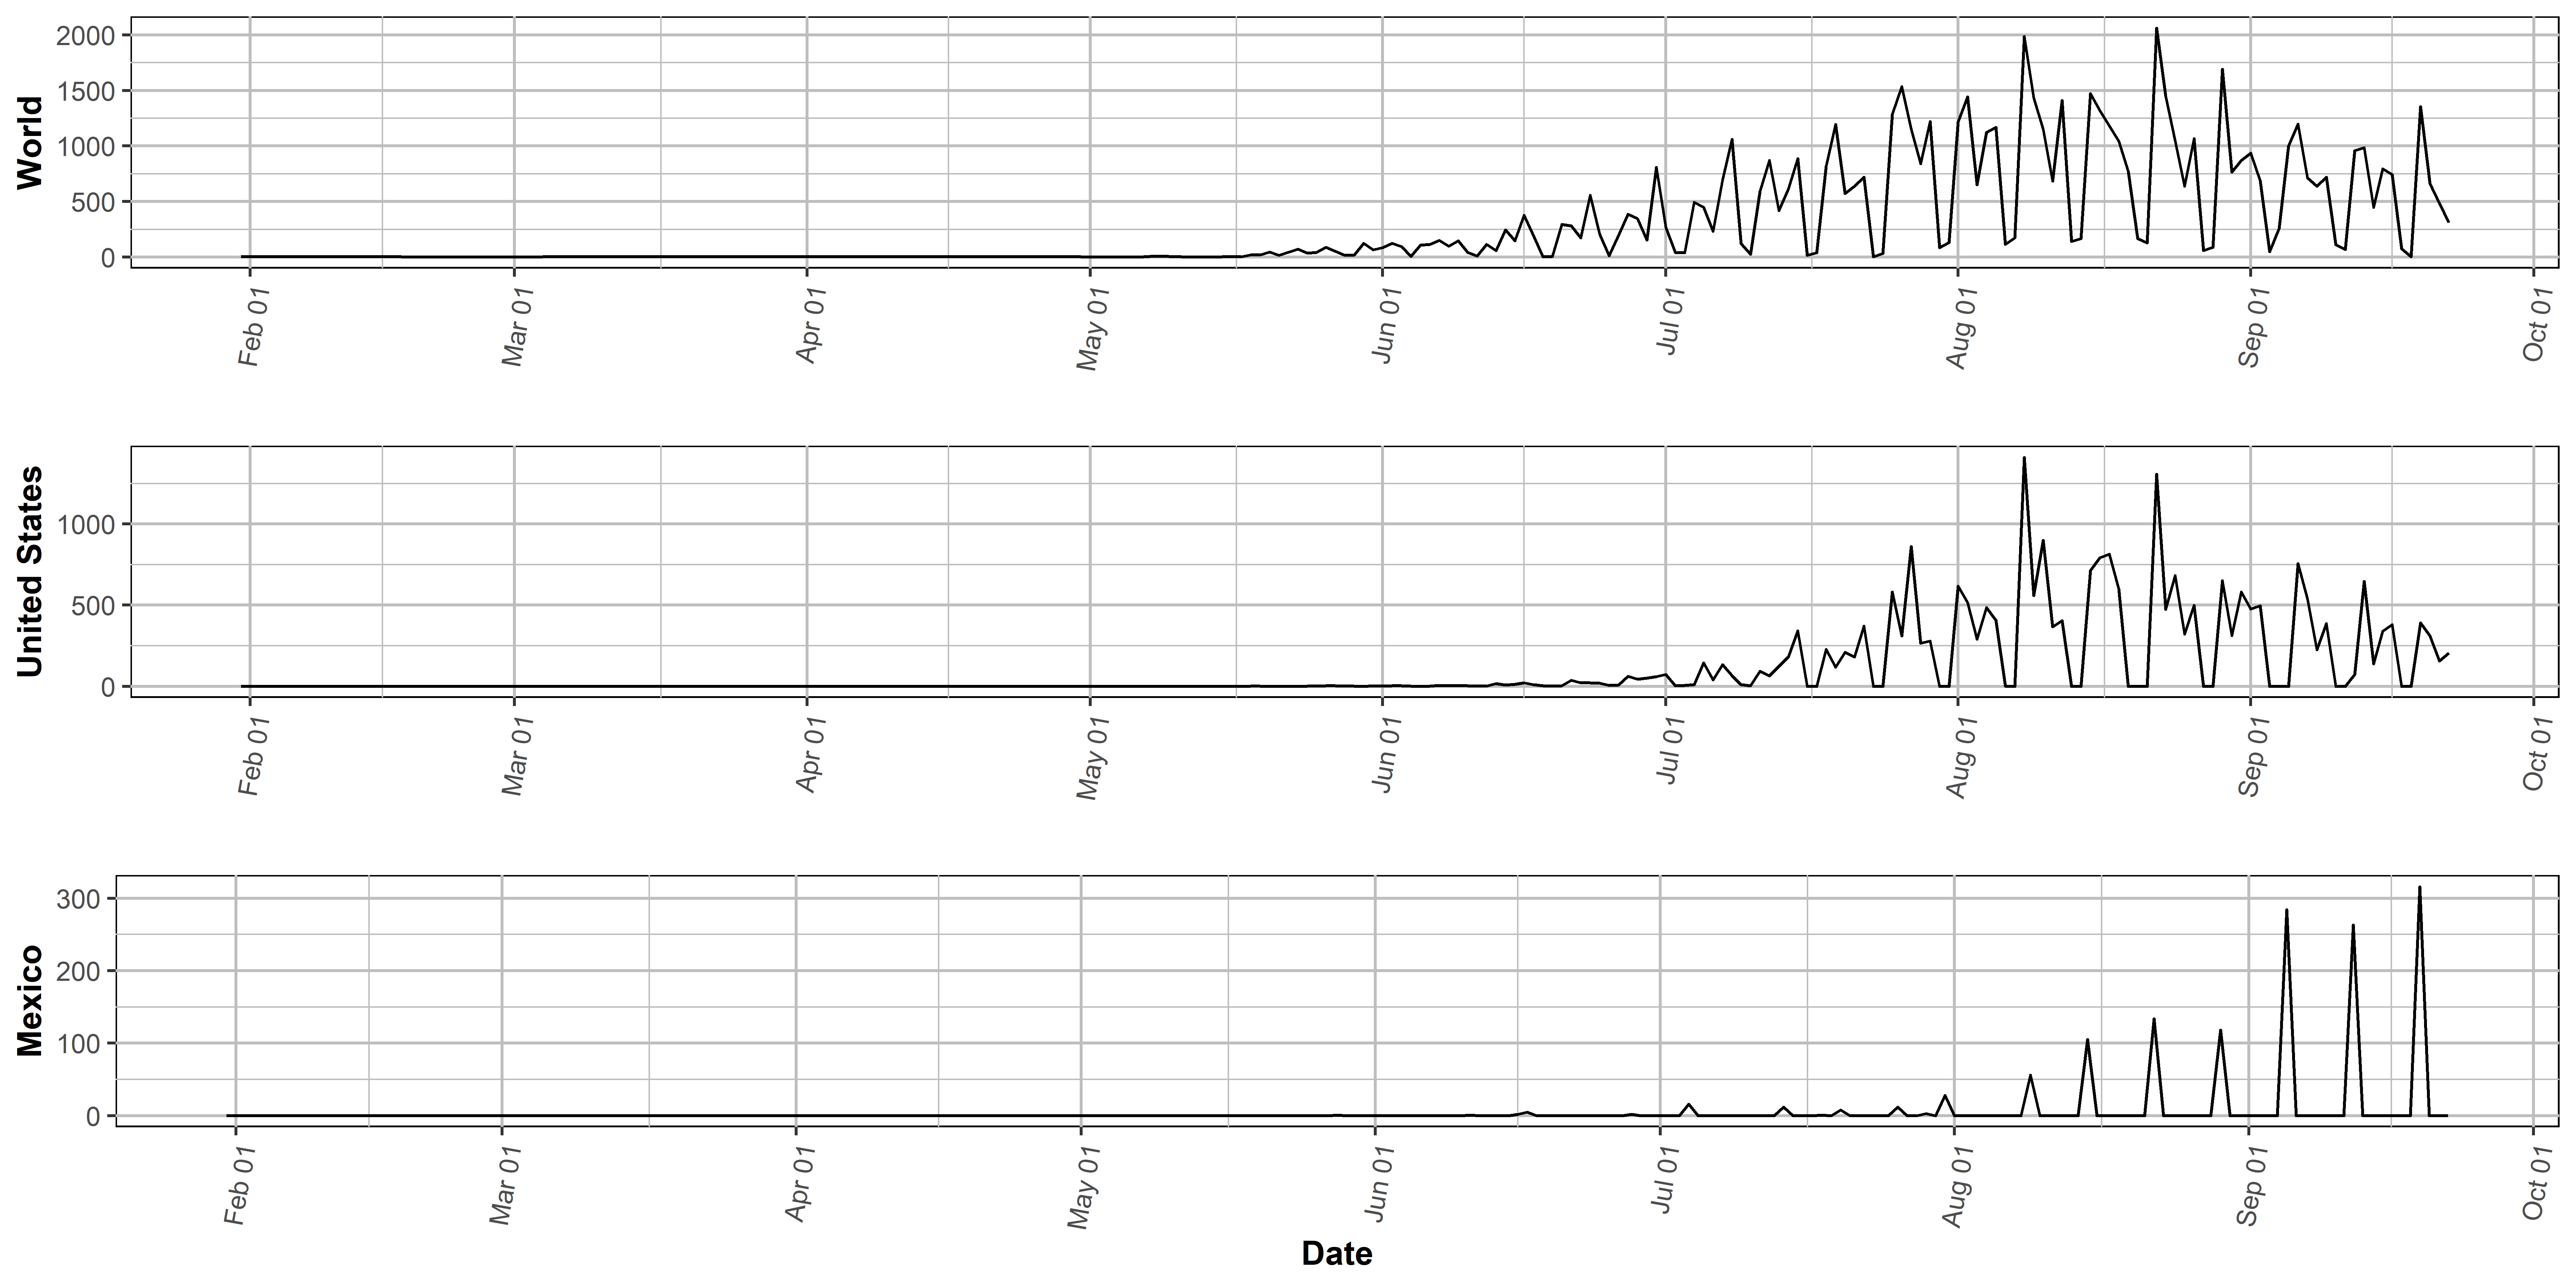
\includegraphics[width = 8 cm]{TimeSeries.png}
    \caption{TS of the World, USA, and Mexico MPX confirmed cases, analyzed from 2022 Kaggle MPX Database~\cite{Contractor2022}}
    \label{fig:MexicoTimeSeries}
\end{figure}

The decomposition of confirmed cases around the world represented in Figure \ref{fig:WorldDecompose} considers the data in the upper part as seen in Figure \ref{fig:MexicoTimeSeries}, with a characteristic trend that begins to increase from the first weeks with a peak at week 14, followed by a decrease until the last weeks. Seasonality and errors are also represented in the lower part of the figure.

%Figure #5
\begin{figure}[H]
    \centering
    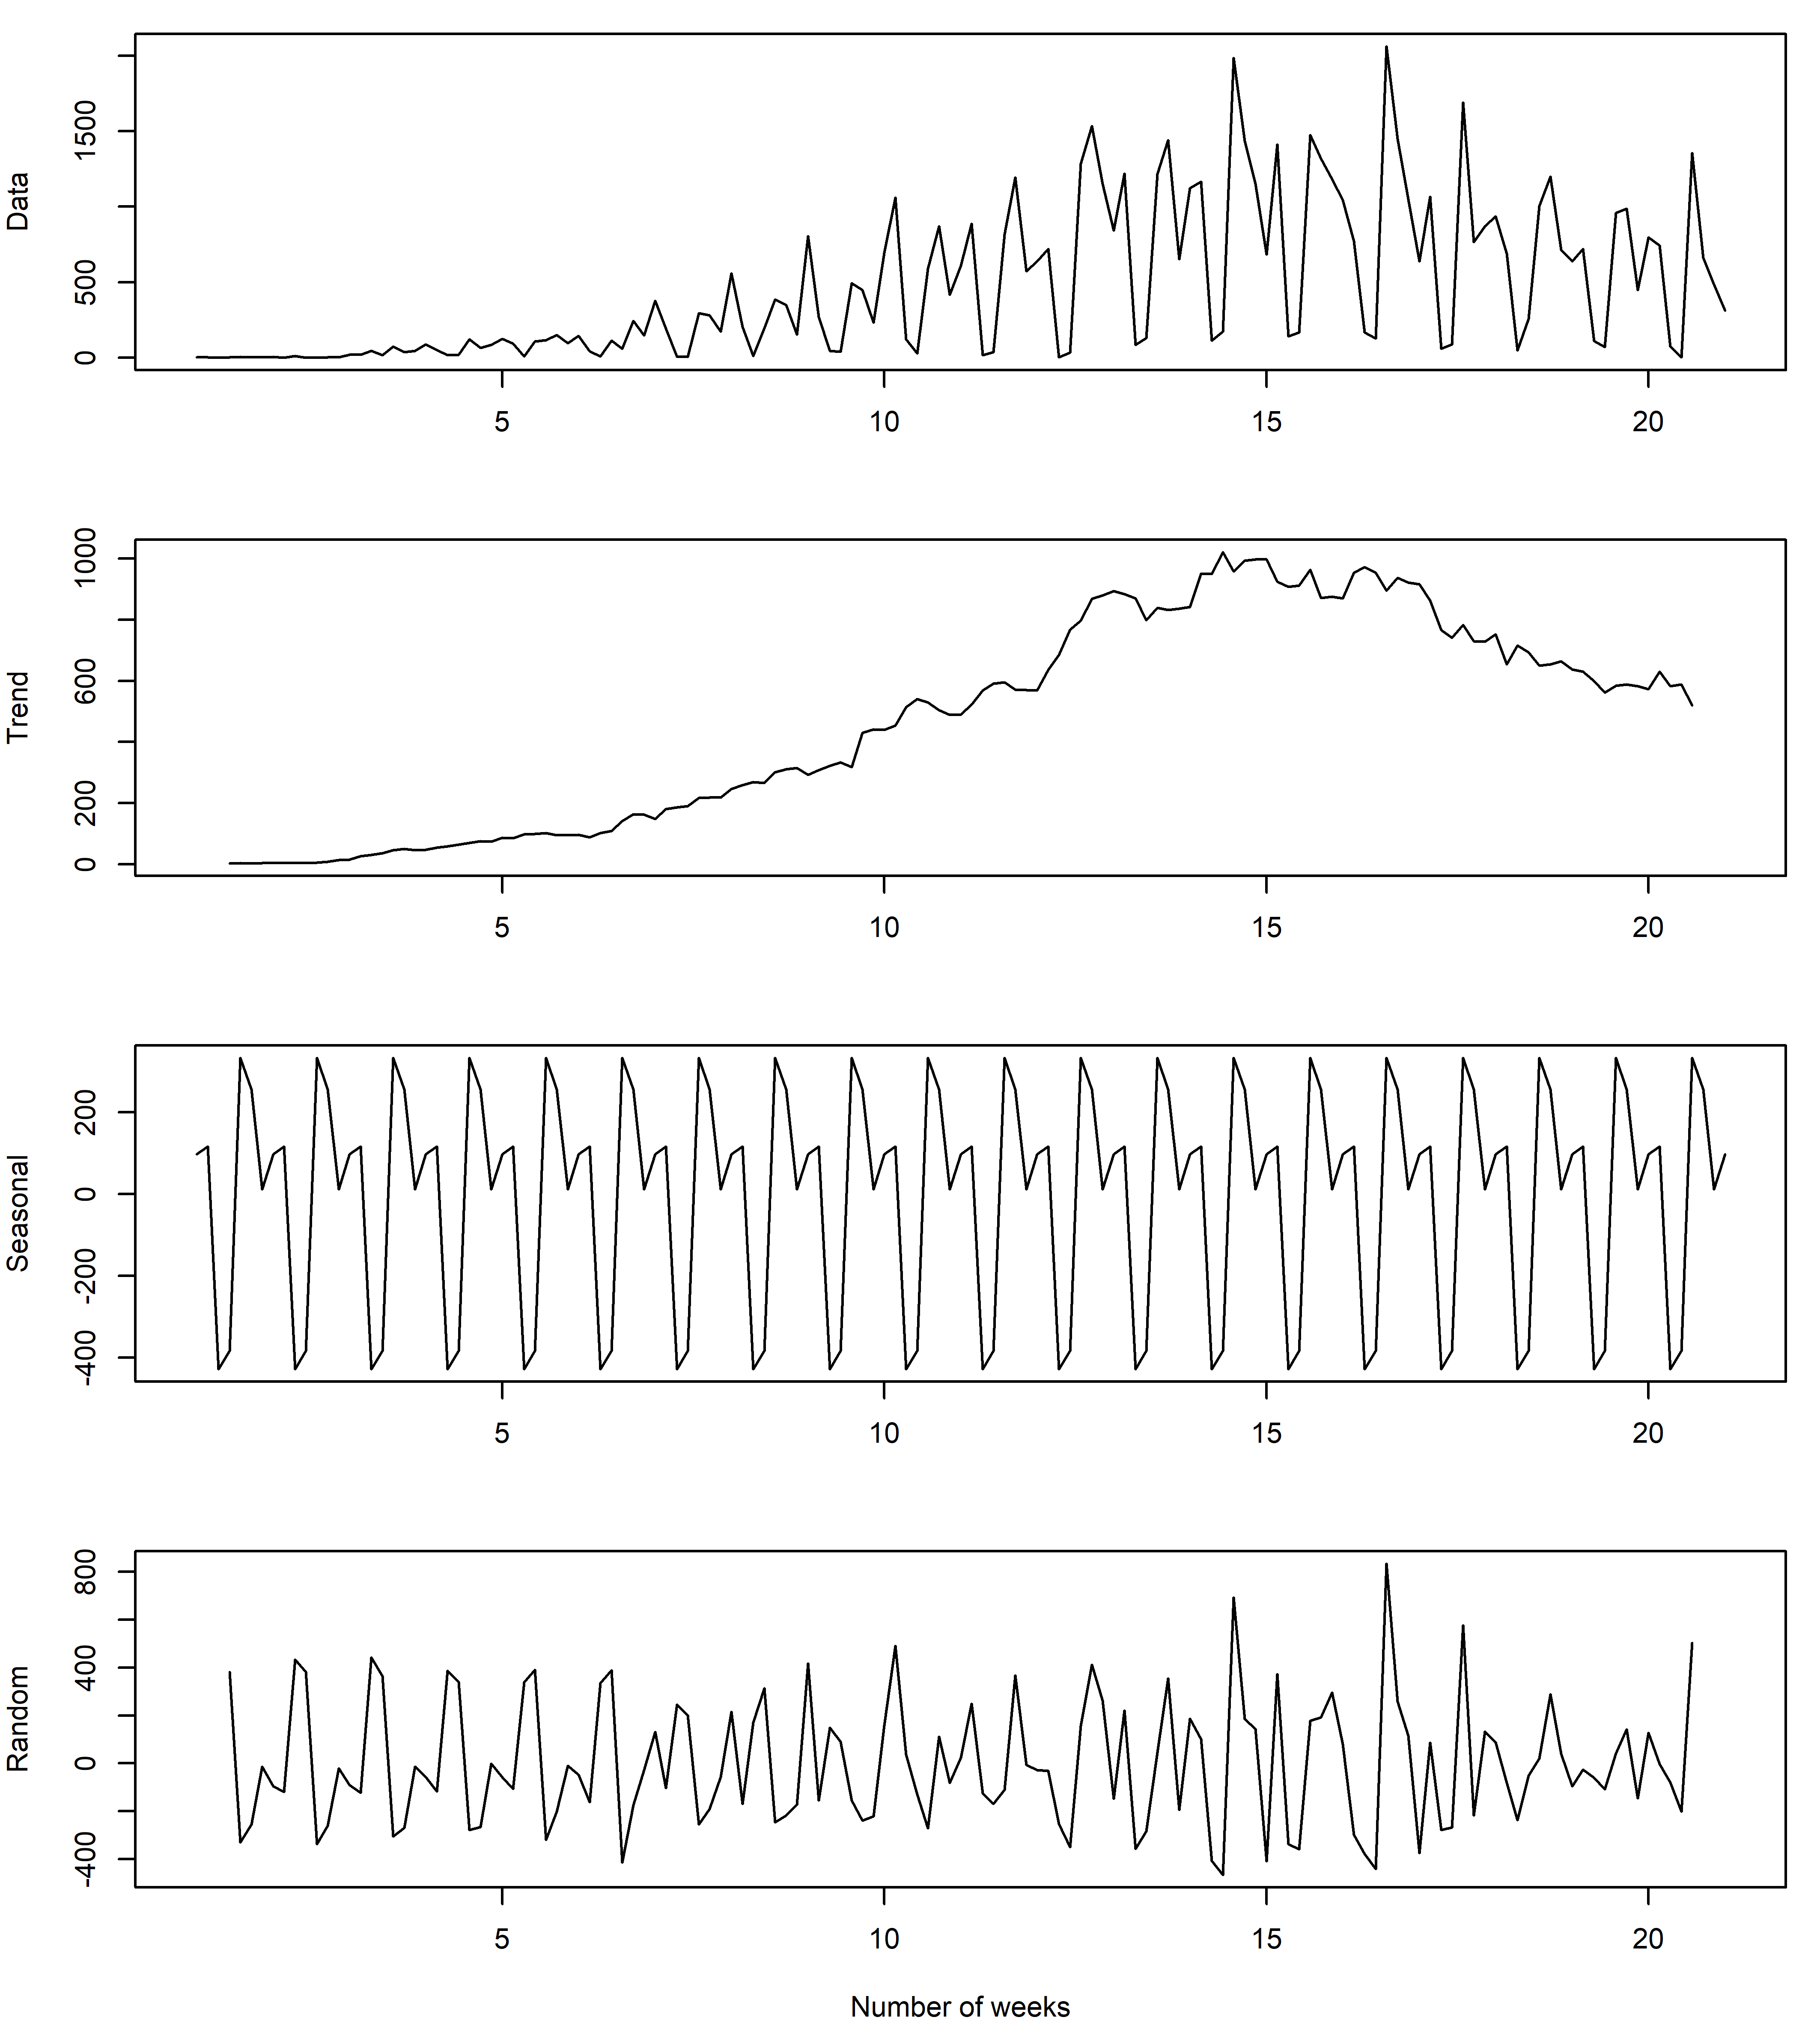
\includegraphics[width = 6 cm]{World_Decompose.png}
    \caption{Decompose of the world MPX confirmed cases TS, analyzed from 2022 Kaggle MPX Database~\cite{Contractor2022}}
    \label{fig:WorldDecompose}
\end{figure}

As seen in the global cases, figure \ref{fig:USADecompose} represents the decomposition of the USA cases where the data behavior and the trend are very similar, as stated before. While the behavior is identical, it started later than the one with the global cases, and the peak for this country was reached at the same time, around weeks 14 and 15, followed by a decrease, even more pronounced than the global cases. Also, seasonality and errors are observed in the lower part of the figure.

%Figure #6
\begin{figure}[H]
    \centering
    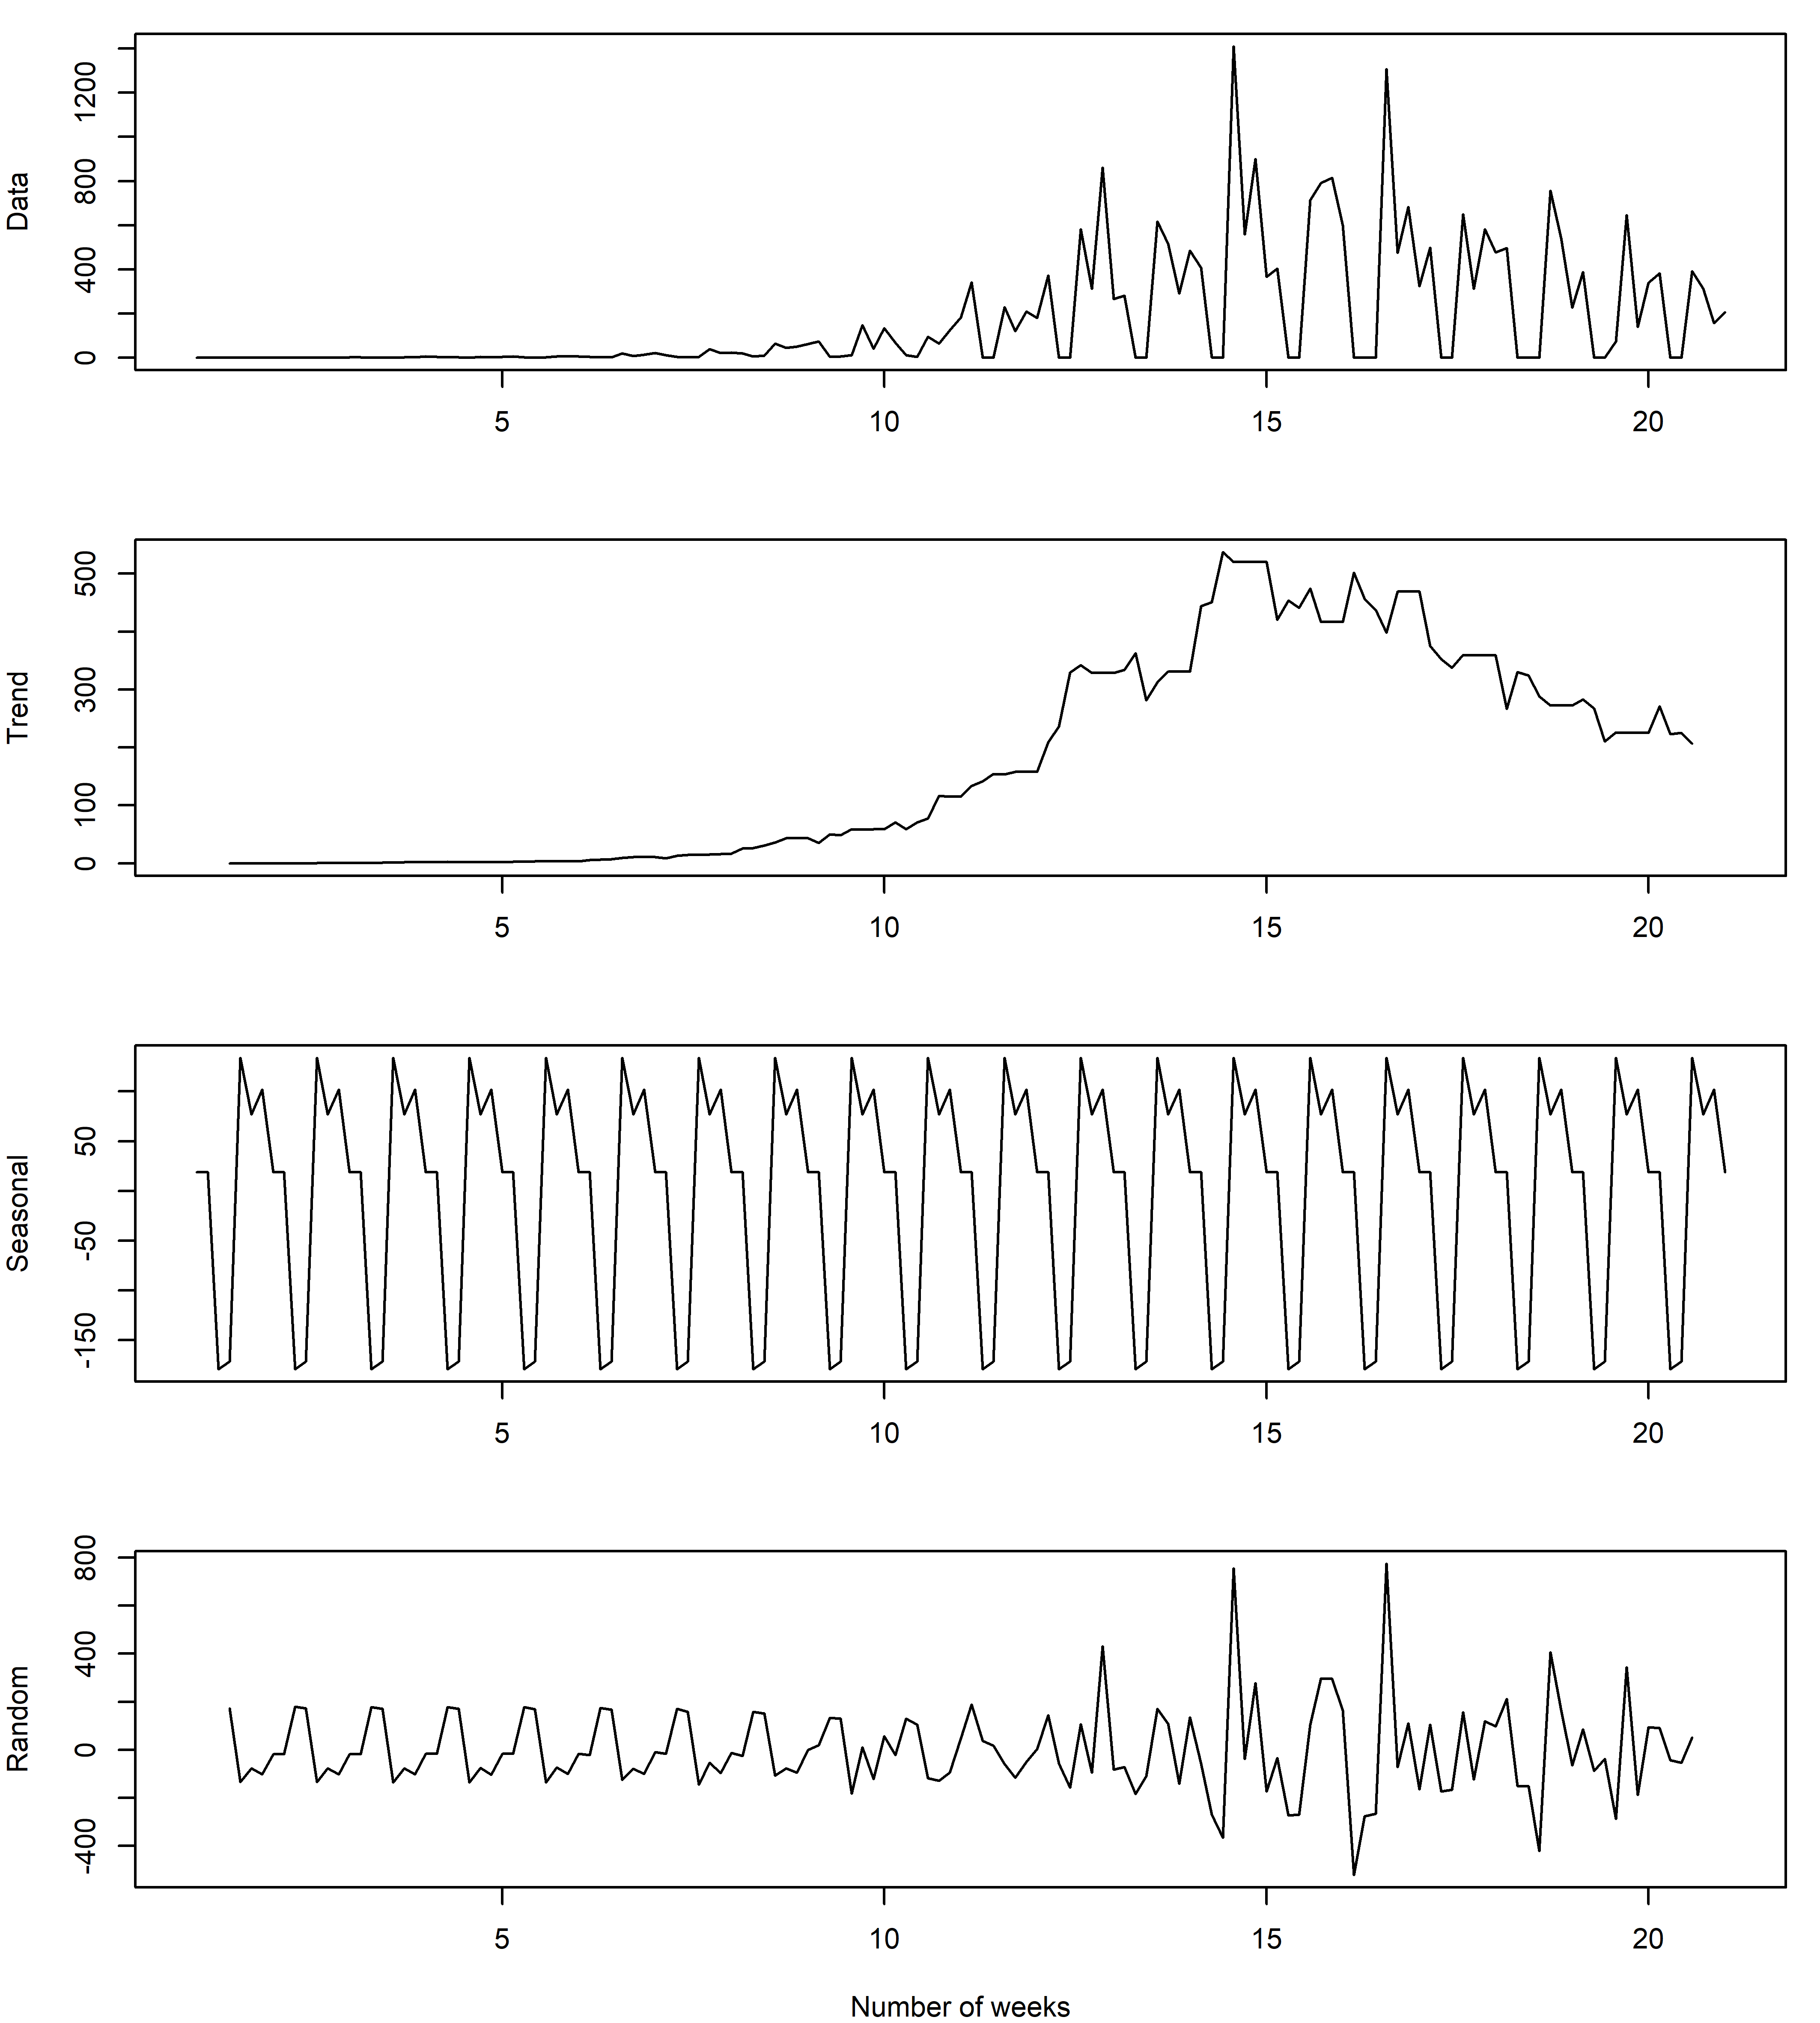
\includegraphics[width = 6 cm]{USA_Decompose.png}
    \caption{Decompose of the USA MPX confirmed cases TS, analyzed from 2022 Kaggle MPX Database~\cite{Contractor2022}}
    \label{fig:USADecompose}
\end{figure}

Lastly, the decomposition of the Mexico TS is shown in~\ref{fig:MexicoDecompose}; compared to the world and the decomposition of the USA, dissimilarities can be observed. The trend component increases continuously over time. Also, the seasonal part of the TS displays one single and sharp peak per weak, and the random element is maintained below zero and repetitive until week 15; after that, explosive behavior is observed.
%Figure #7
\begin{figure}[H]
    \centering
    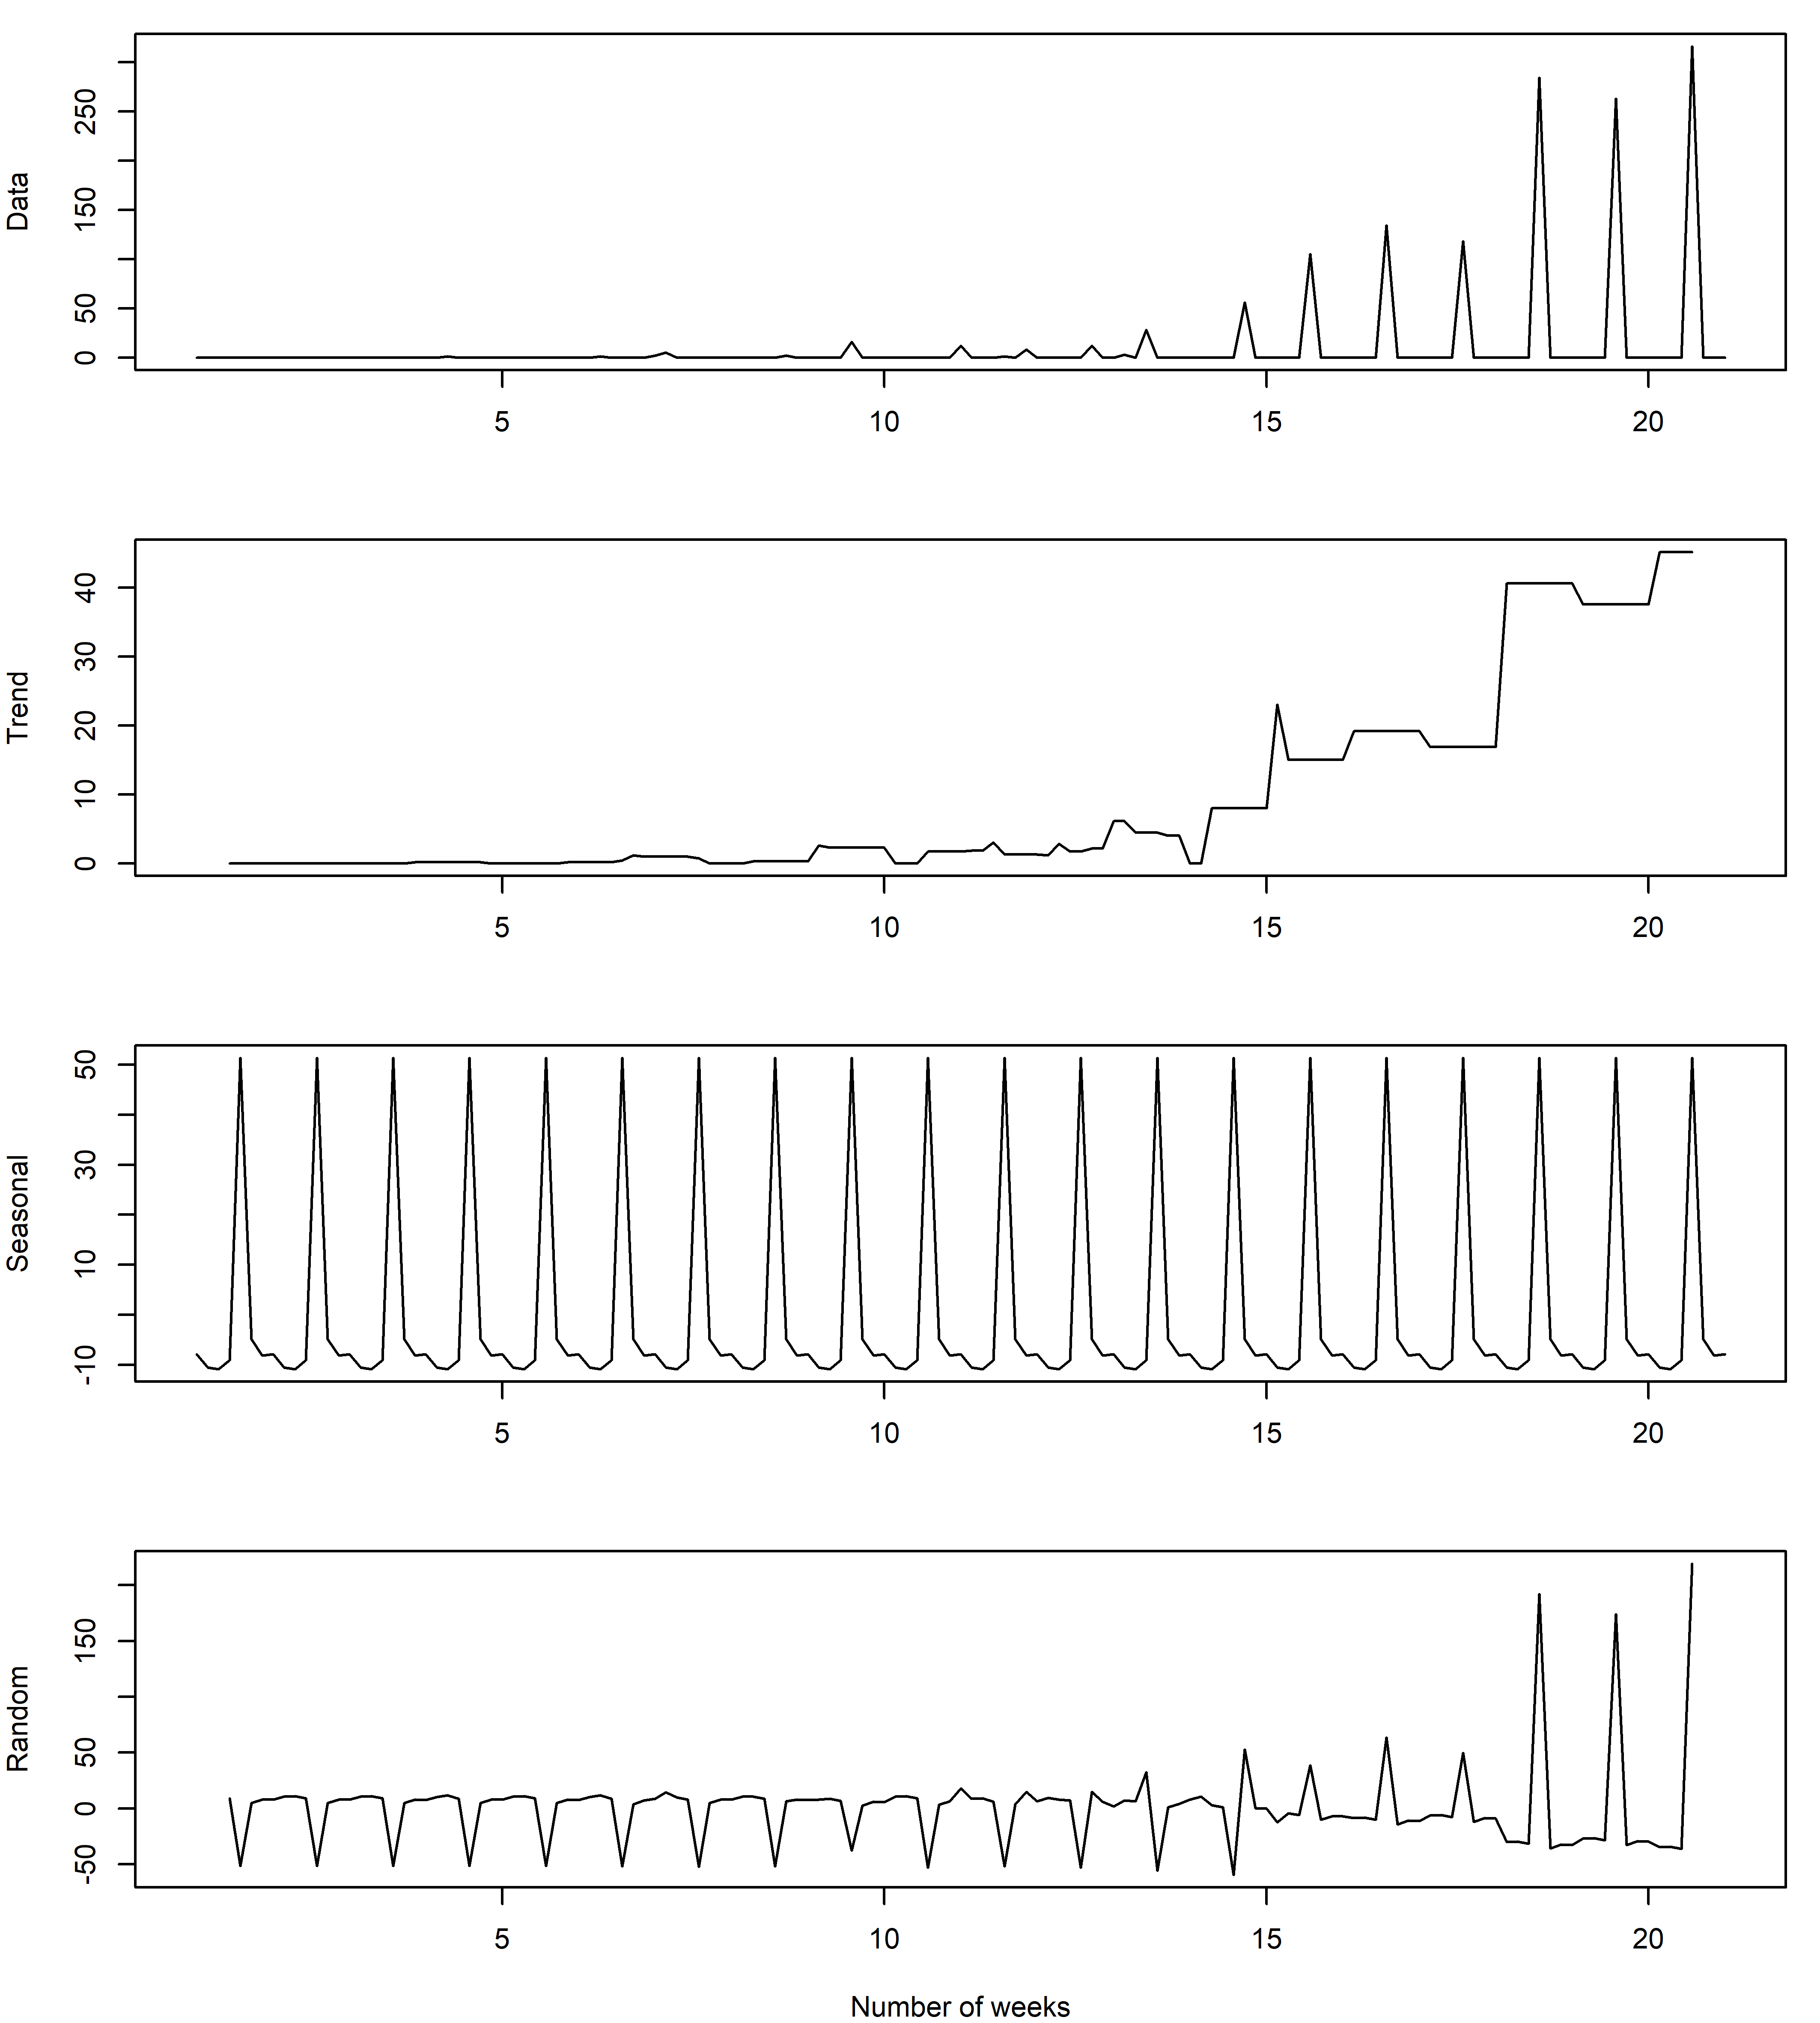
\includegraphics[width = 6 cm]{Mexico_Decompose.png}
    \caption{Decompose of the Mexico MPX confirmed cases TS, analyzed from 2022 Kaggle MPX Database~\cite{Contractor2022}}
    \label{fig:MexicoDecompose}
\end{figure}

The ARIMA model (p,d,q) used for Mexico was ARIMA (4,1,3), with an AIC of 1412.04 and a BIC of 1438.51. The result was smaller than the world and the USA coefficients. The parameters of the models are represented in Table~\ref{Table:parameters}.

%Table #1
\begin{table}[h!]
    \centering
    \caption{Parameters of the ARIMA model.}
    \label{Table:parameters}
    \begin{tabular}{|c|c|c|c|c|}
    
    \hline
        Region & ARIMA model &  AR, MA coefficient & AIC & BIC\\
    \hline
        World & (2, 1, 1) & -0.4152, -0.8525 & 2,060.92 & 2072.69\\
    \hline
        USA & (0, 1, 1) & 0, -0.8842 & 1,927.37 & 1933.26\\   
    \hline
        MEX & (4, 1, 3) & -0.48, 0.71 & 1,412.04 & 1,438.51\\
     \hline
    \end{tabular}
\end{table}

The difference in data was transformed into stationary data by stabilizing the mean daily cases from Figure~\ref{fig:MexicoTimeSeries}. Adjusted data can also be seen in Figure~\ref{fig:Differences}. 
%Figure #8
\begin{figure}[H]
    \centering
    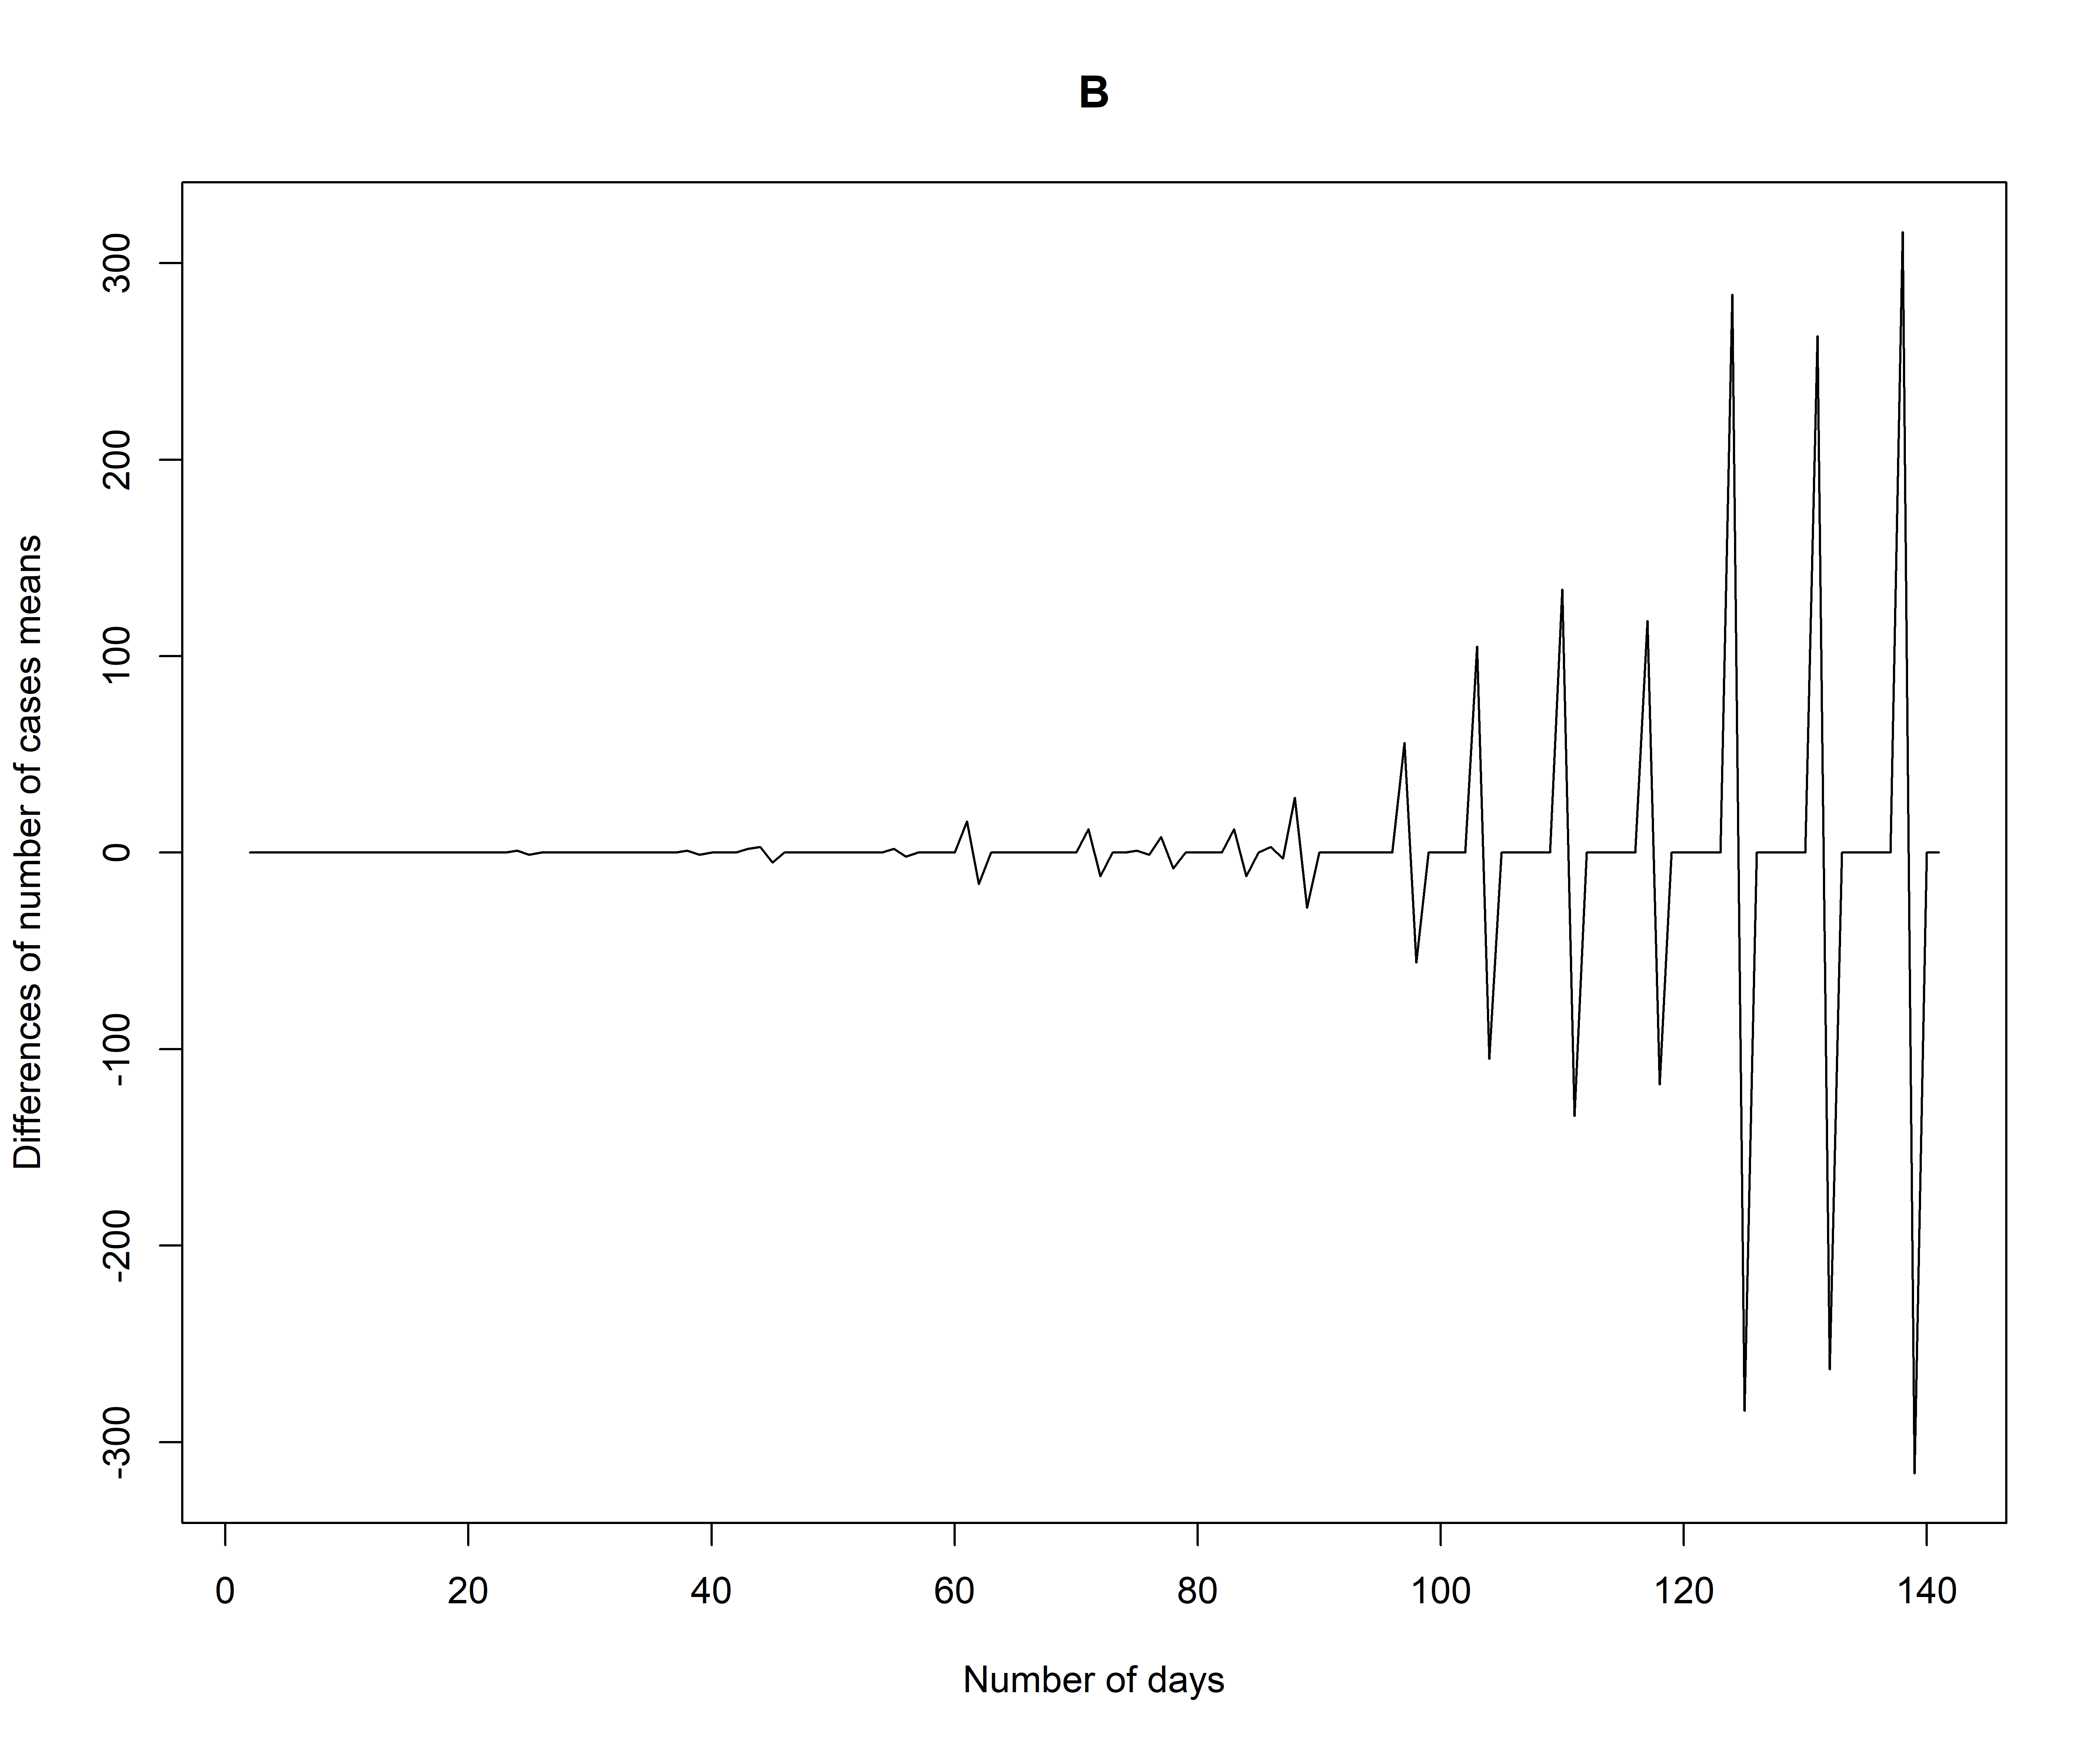
\includegraphics[width = 8 cm]{Differences.png}
    \caption{Difference of the TS of Mexico MPX cases represented by day count, analyzed from 2022 Kaggle MPX Database~\cite{Contractor2022}}
    \label{fig:Differences}
\end{figure}

To support the differencing of the TS and the model parameters, the autocorrelation function (ACF) was applied and represented in Figure~\ref{fig:ACF&PACF}-A. The ACF correlates the different past values concerning the following matters. The partial autocorrelation function (PACF) represented in Figure~\ref{fig:ACF&PACF}-B measures the degree of relationships between lag and variable.
%Figure #9
\begin{figure}[H]
    \centering
    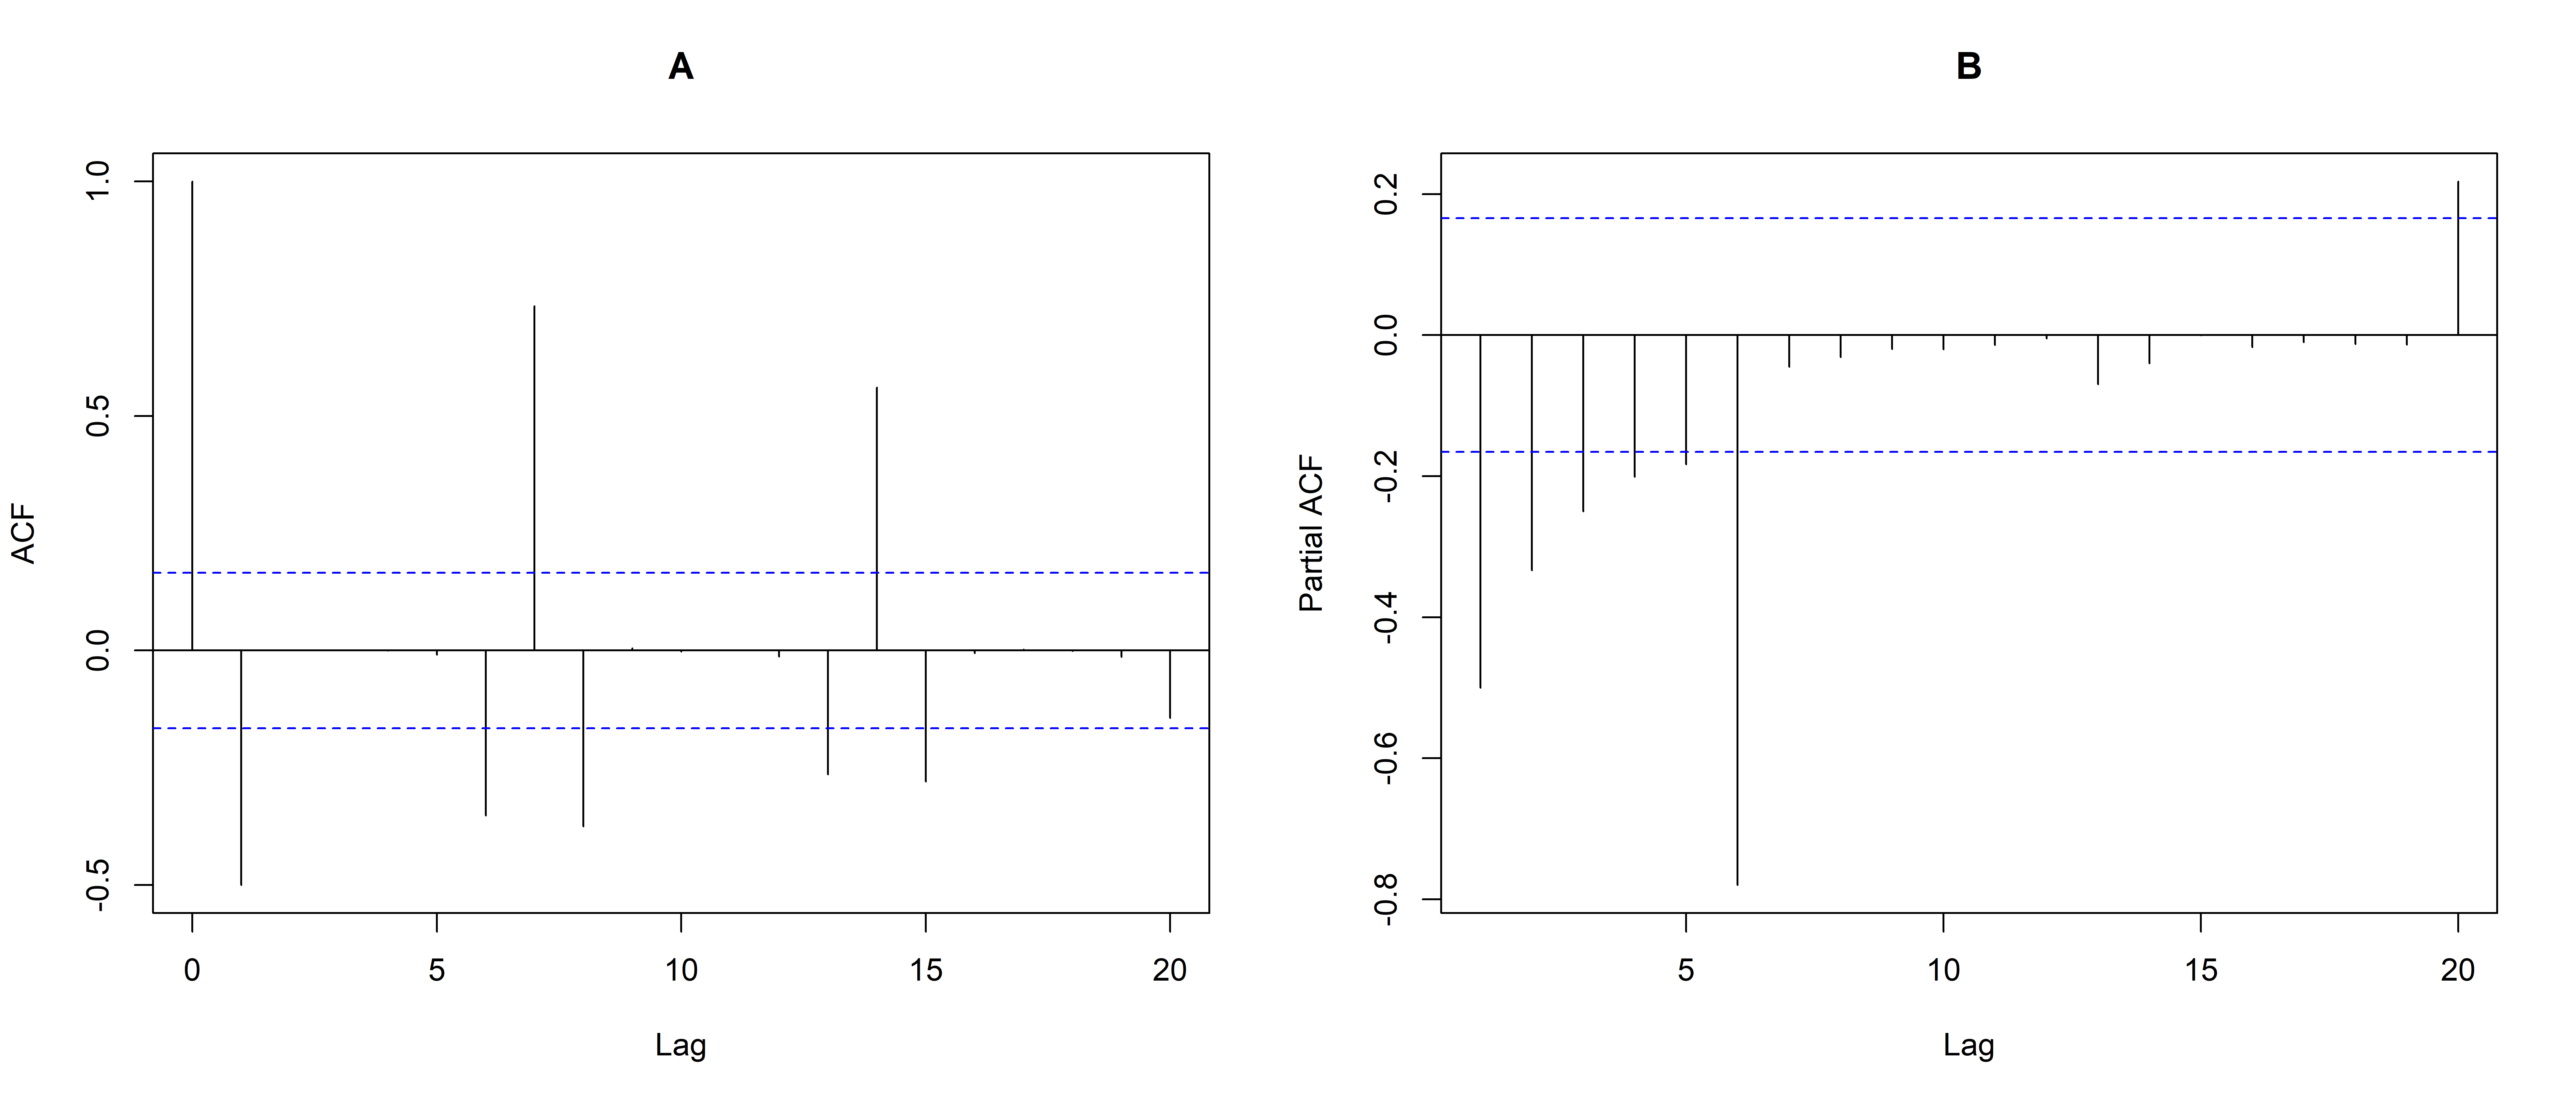
\includegraphics[width = 8 cm]{ACF&PACF.png}
    \caption{Analysis related to seasonality and stationarity, analyzed from 2022 Kaggle MPX Database~\cite{Contractor2022}}
    \label{fig:ACF&PACF}
\end{figure}

With the Mexico model, the forecast for the next 15 days was calculated and represented in Figure~\ref{fig:Forecast&Residuals}-A. In general, the trend shown by the model is a slight reduction for the cases of the following weeks. For the validation of this model, the residuals resulting from the predicted values were represented and analyzed in Figure~\ref{fig:Forecast&Residuals}-B. 
%Figure #10
\begin{figure}[H]
    \centering
    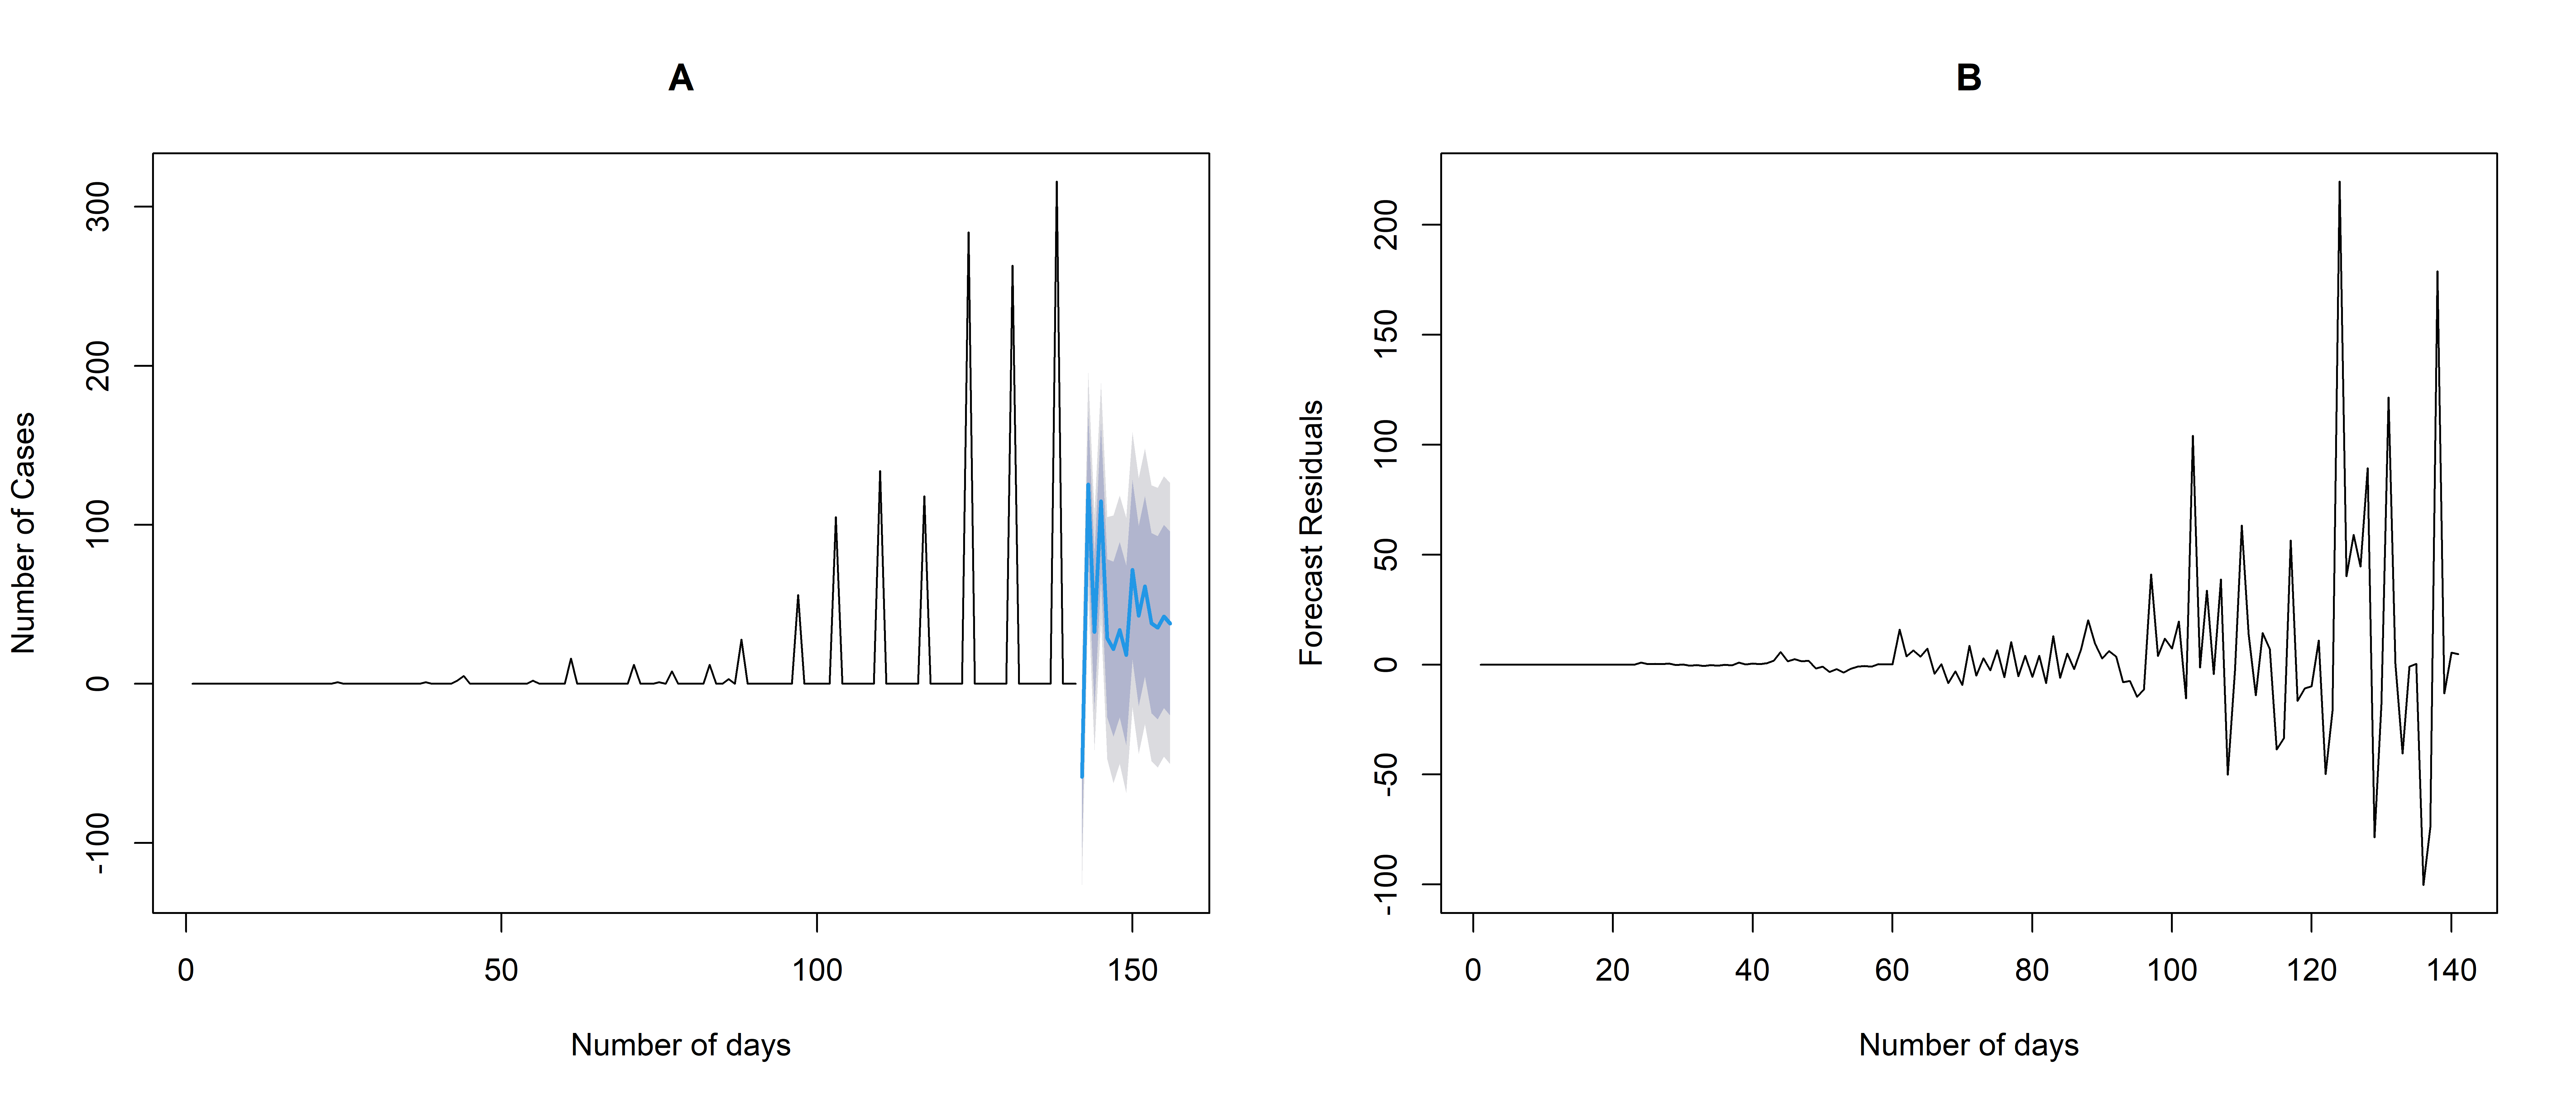
\includegraphics[width = 8 cm]{Forecast&Residuals.png}
    \caption{A) TS Predictions of Mexico MPX cases represented by day count, B) Resulting residuals of the forecasts from Mexico MPX cases represented by day count, analyzed from 2022 Kaggle MPX Database~\cite{Contractor2022}}
    \label{fig:Forecast&Residuals}
\end{figure}

The model predicts values ranging from 0 to 125 cases for the next day. In Table~\ref{Table:Forecasting}, the prediction values are displayed, with a lower limit showing that most lower limits reach 0 cases and an upper limit reaching values up to 171 cases.
%Table #2
\begin{table}[h!]

    \centering
    \caption{Prediction of MPX cases for the next 15 days.}
    \label{Table:Forecasting}
    \begin{tabular}{|c|c|c|c|}
    
     \hline
        Day &  Forecast & lower limit & Upper limit\\
     \hline
       1 & 0 & 0& 0.00\\
       2 & 125.55 & 79.70& 171.40\\
       3 & 32.61 &0 & 81.11\\
       4 & 114.98 &66.44 & 163.53\\
       5 & 28.76 &0 &78.56 \\
       6 &21.76 & 0&76.81 \\
       7 &34.04 & 0& 89.18\\
       8 & 18.04& 0& 74.58\\
       9 &71.77 &15.21 & 128.34\\
       10 & 42.73&0 & 99.41\\
       11& 61.33&4.59 & 118.08\\
       12 & 38.19&0 & 94.93\\
       13&35.36 & 0& 92.89\\
       14&42.40 & 0& 100.02\\
       15 & 37.89&0 & 95.71\\
     \hline
    \end{tabular}
    
\end{table}

A histogram of the forecast errors was constructed; the data were generated with mean 0 and standard deviation. The histogram of the forecast errors is colored red with the overlaid distributed data. This curve is blue at the top of the forecast error histogram. The successive forecast errors usually appear distributed; therefore, ARIMA (4, 1, 3) may be an adequate model for MPXV cases. These results can be seen in Figure~\ref{fig:HistErrors}. 
%Figure #9
\begin{figure}[H]
    \centering
    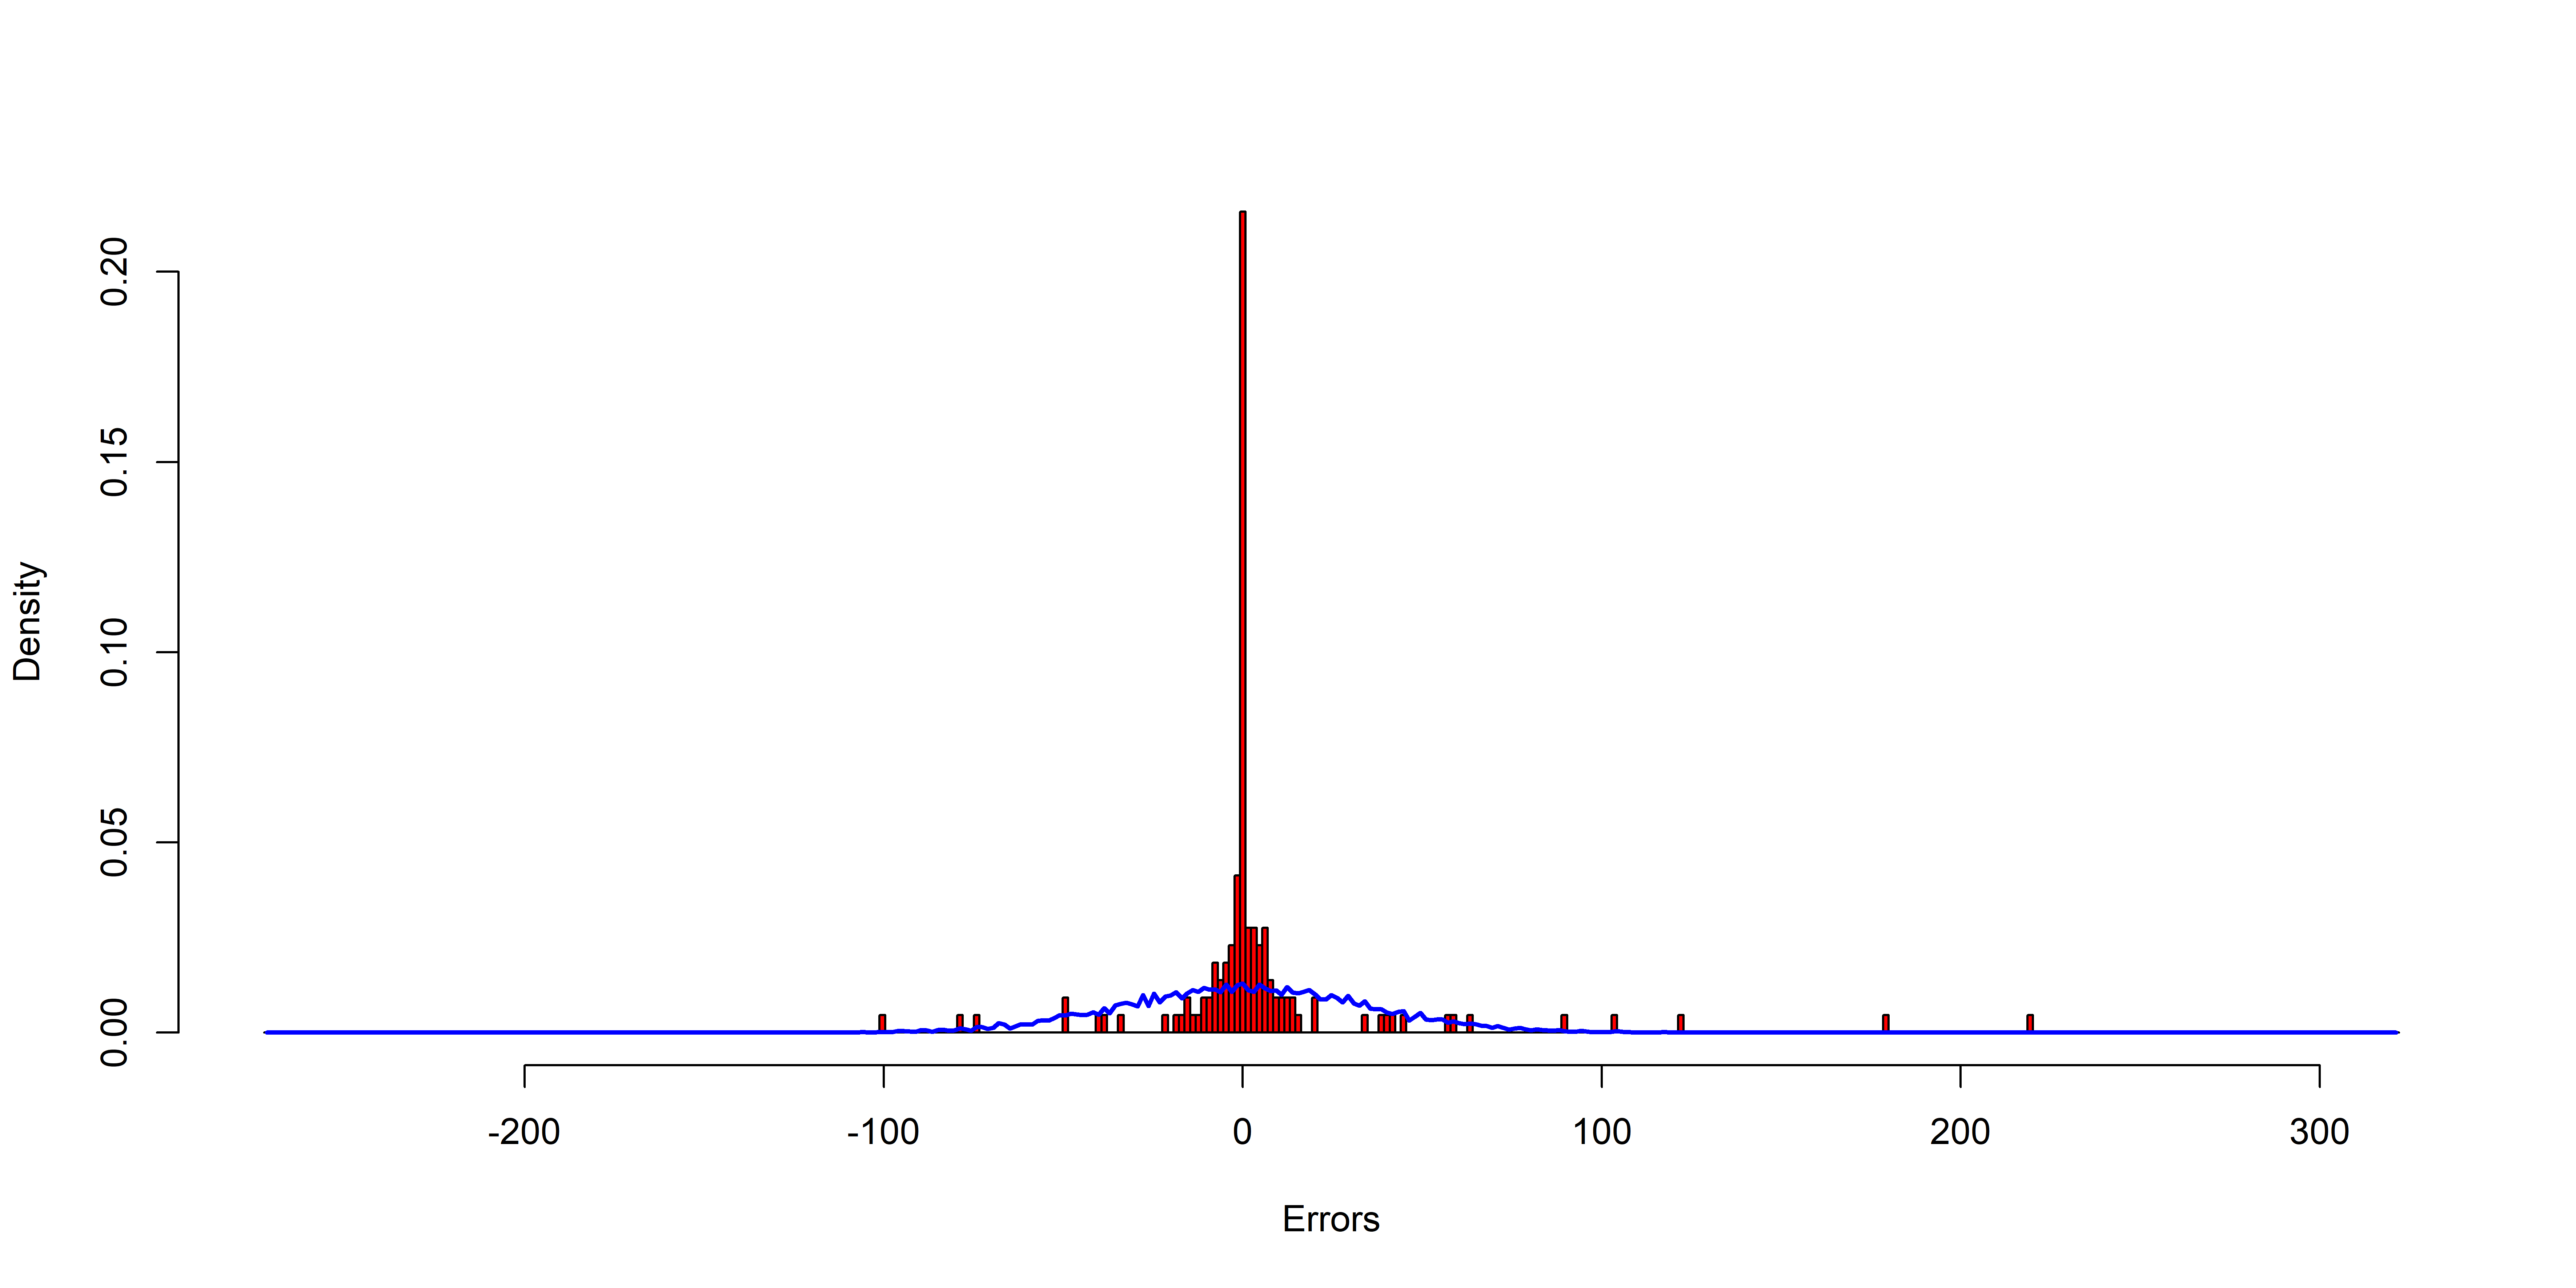
\includegraphics[width = 8 cm]{HistErrors.png}
    \caption{The errors of the Arima model forecast plotted as a distribution, the curve with the actual distribution is in the color blue, analyzed from 2022 Kaggle MPX Database~\cite{Contractor2022}}
    \label{fig:HistErrors}
\end{figure}

\section{Discussion}

In this study, the analysis of the MPX case data set was analyzed using an ARIMA model. The model was developed by using the "autoarima" function in RStudio, and with this model, we selected the parameters used for forecasting. The model predicted cases with a lower and an upper limit for the next 15 days. With this information, the government and several institutions can prepare a pandemic strategy, make informed decisions that can benefit the population, and, in particular, take care of people who may be at risk if they become infected. 

The Mexican cases had better results than the model adjusted for the global and the USA cases. In the three models, the residuals present a normal distribution. As more data are added to the record of points in Mexico, better prediction and understanding of the MPX outbreak will be achieved. Regarding the difference in the decomposition analysis, the trend of the USA and the Global cases present huge similarities, whereas, in the Mexican graph, we see a different direction. The behavior could be other because the number of cases is substantially lower, and the first cases started several days after the global and USA issues. Still, the Mexican trend may take the same form as the international and USA trend as time passes.

Other studies have used this time series analysis methodology with an ARIMA model to predict epidemiological data. In particular, Ceylan Zeynep indicates the prevalence of COVID-19 in 3 different countries, Italy, Spain, and France, using the ARIMA model and comparing them better to understand the behavior of the outbreak~\cite{Ceylan2020}. However, this type of analysis was not previously conducted for MPXV cases. This study is the first milestone in studying MPXV cases to prevent them from escalating into a more severe situation.

\section{Conclusion}
The observed results are proof that time series analysis is a powerful tool that can be used to predict and prevent. It has been used to model information on epidemiological data and to obtain models with valuable information on the current situation that is expected in the future. This study analyzed MPX cases worldwide, in the United States and Mexico. It also presents predictions for MPX cases in Mexico for the next 15 days. The projections have a slight tendency to decrease over the next few weeks; however, there is no visible end in sight for the MPX cases in Mexico. This information needs to be continually updated for better results. For future work, this approach can be applied to other countries where the cases have different trends to compare the socioeconomic and political contexts and to help governments or institutions in their decision-making process. This model can be integrated with other computational approaches to improve predictions and reduce data uncertainty, prevent the MPXV outbreak from escalating, and also serve as a tool to predict and prevent other merging diseases from becoming a brutal pandemic. 

\bibliographystyle{plain}
\bibliography{AM_FPA_References.bib}

\end{document}